\chapter{Evaluation}
This chapter provides a description of the Evaluation test bed for the OpenVswitch-Event Processing System and a brief discussion of the results.

\section{Evaluation Testbed}
The system under test is the OpenVswitch userspace bridge. To set up the evaluation test bed, two network Namespaces are created and connected to the OpenVswitch bridge running in userspace mode. Namespace A runs a Java UDP event generator application, which is bridged via OpenVswitch - the system under test, to another Java application consuming the events in Namespace B, thereby simulating a Networked environment. The application at A timestamps the datagram before Send, for the application at B to compare the time stamp on Receive to get the point-to-point latency, which is aggregated over ${10^5}$ datagrams to get the latency.

\section{Parameters for Evaluation}
Two parameters are initially considered for the evaluation, namely, a) The measure of latency against rules with increasing size of event type field. b) The measure of latency against percentage of datagrams filtered on event type field.
\subsection{Size of Event Type}
As described in the system model, Event Type is a string field present in the first position of an event payload. The effects of performing a match on event type field with varying lengths to point-to-point latency is measured and the results are illustrated below in Figure 1.\newline
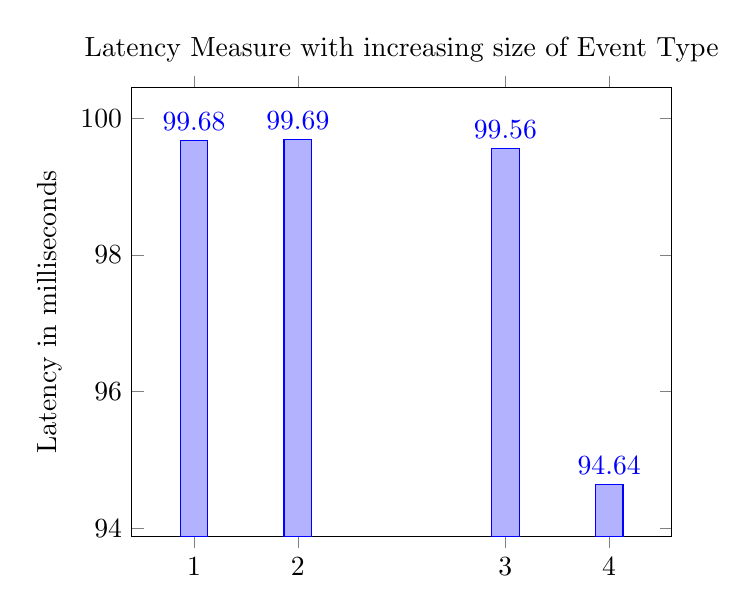
\begin{tikzpicture}
\begin{axis}[
title=Latency Measure with increasing size of Event Type,
ybar,
enlargelimits=0.15,
legend style={at={(0.5,-0.25)},
	anchor=north,legend columns=-1},
ylabel={Latency in milliseconds},
symbolic x coords={1,2,,3,4,5,6,7,8,9},
xtick=data,
nodes near coords,
nodes near coords align={vertical},
]
\addplot coordinates {(1,99.68)(2,99.69)(3,99.56)(4,94.64)(5,)(6,)(7,)(8,)(9,)};
%\addplot coordinates {(5,7.61)(10,7.79)(20,9.2)(40,25.05) };
%\addplot coordinates {(5,44.2)(10,63.2)(20,94.8)(40,118.3) };
%\legend{No. of flows,1ms delay,CPU LOAD}
\end{axis}
\end{tikzpicture}
 
The increasing size of event type string doesn't result in a linear increase in latency. This is explained by the fact that Tuple search space classifier of OpenVswitch creates a Hash table for every unique combination of inserted flow rule. In the case of this evaluation, one flow rule is added for each run, while increasing the size of event type field in consecutive runs. Additionally, although the event type field matches against a string in the event payload, the match field during flow rule insertion for event type is Hexadecimal value of the string. The rationale behind this approach is that strings within an event payload are serialized into Hexadecimal values on the wire, and since Event Parsing is part of the packet processing pipeline, keeping the fields as-is avoids the expensive conversion, thus reducing the overhead to the pipeline. So, to match an event payload with the an event type of 'A', the match field in the rule, 'e_type=0x41'

Figure 1 also contrasts the latency of an event type match with the latency measured for transport header match in OpenVswitch Master release 2.6.1 userspace bridge and a similar match on OpenVswitch-Event Processing(OVS-EP) bridge. The results show that the OVS-EP bridge adds a small latency even when the match levels are the same. This is because, the OVS-EP implementation has an Event Parsing layer part of the packet processing pipline and supports additional fields for matching on an Event Payload.

\subsection{Percentage of Flows Filtered}
Another interesting parameter that is evaluated is the rate of change of latency as increasing percentage of events are filtered. The results are illustrated in Figure 2.\newline
\newline
\newline
\newline
\newline
\newline\newline
Latency measure on Filtered Flow percentage
\newline
\newline
\newline
\newline\newline
\newline
\newline

 The important difference in the evaluation is that the event generator generates events for 10 different event types, and ten flow rules are added to explicitly forward these types. To begin the evaluation the flow rules for each type are modified to filter the event of those types only. So, we begin with ten flow rules with the NORMAL action and change the action to DROP as we progress through the evaluation. The results show that as flow rules are inserted to increase the percentage of filtered events, the latency remains steady. This is because the number of flow rules remain constant, only the actions on each flow rule is modified to increase filtered events. And since the Tuple Space Search Classifier only adds an additional Hashtable when there is an new combination of fields entered as a flow rule, even increasing the number flow rules, as long as they have the same match fields would not result in additional lookups.

